% =============================================================================
% Section 1: Introduction
% =============================================================================
% PURPOSE:
%   Frame the capstone around a general inverse-problem principle rather than
%   as a programme summary.  Emphasise the gap between forward adequacy and
%   inverse adequacy, identify geometry/asphericity as the controlling
%   mechanism, and position the companion applications as evidence.
% =============================================================================

\section{Introduction}
\label{sec:introduction}

Spectral inverse problems arise whenever one seeks to infer physical
parameters from observed resonances.  Structural dynamics, elastographic
parameter recovery, and non-destructive testing all use the same basic logic:
one posits a forward model, matches its predicted frequencies to measured
ones, and then estimates the parameters that minimise the residual mismatch
~\cite{Gladwell2004,Gladwell2005,MottersheadFriswell1993,FriswellMottershead1995,Doyley2012}.
For simple geometries this approach can be highly effective.  Yet its success
also invites a dangerous inference.  A forward model that reproduces the
spectrum accurately need not define a well-posed inverse map.  Forward
adequacy does not guarantee inverse adequacy.

That distinction is central to classical spectral theory.  Kac's question ---
``Can one hear the shape of a drum?'' --- remains influential precisely because
it asks what spectral data do and do not determine~\cite{Kac1966}.  The later
construction of isospectral but non-congruent domains did not make inverse
spectral analysis irrelevant; it made the role of symmetry impossible to
ignore~\cite{Gordon1992}.  The present setting is not the Laplacian drum problem itself, but a coupled fluid--structure spectral inverse problem in which the same symmetry question reappears in practical form.  The relevant question is often not
whether uniqueness holds globally, but whether the measured spectrum contains
enough locally independent information to separate geometry from material
properties at the operating point of interest.

In this paper we study that question for fluid-filled viscoelastic shells.
These systems appear in biomechanics, soft-structure acoustics, and
agricultural sensing, but the present claim is not application-specific.
Our concern is a general mechanism.  A symmetry-reduced shell model may predict
low-order modal frequencies to within a few per cent and therefore appear
entirely satisfactory as a forward description.  The same model may,
nevertheless, be rank deficient for parameter recovery because the reduction
collapses distinct geometric directions into a single scalar surrogate.  In
that case the spectrum still tracks resonance frequencies well, but no longer
separates the curvature and material effects that generated them.  The model is
forward adequate and inverse inadequate.

The mechanism is geometric before it is statistical.  Equivalent-radius or
otherwise symmetry-compressed descriptions are attractive because they preserve
the dominant frequency scale of the shell while simplifying the parameter
space.  What they do not preserve is the full set of curvature channels by
which different flexural modes probe the structure.  When those channels are
collapsed, independent parameter directions become spectrally aligned and the
scaled Jacobian loses rank.  Small forward error may therefore coexist with
catastrophic conditioning of the inverse map.  This is not merely a numerical
inconvenience.  It is a structural consequence of symmetry reduction in a
spectral inverse problem.

The cure is also geometric.  Breaking spherical symmetry in the oblate direction restores mode-specific curvature sampling on a non-singular neighbourhood of the sphere.  Distinct flexural modes then respond
differently to changes in the shell geometry, so the singular value that
vanishes in the spherical limit is lifted once the shell becomes aspherical.
We show this analytically for oblate perturbations of the sphere and numerically
across several fluid-filled shell classes.  The resulting picture is that
asphericity is not a nuisance correction to an otherwise ideal spherical model;
in the present setting, oblate asphericity can restore local practical identifiability.

The broader thesis may be stated in a compact way.  In fluid-filled viscoelastic shells, geometry enters in three logically distinct roles.  It filters
how forcing projects onto admissible deformation fields; it organises the modal
spectrum through curvature, symmetry, and fluid loading; and it determines
whether that spectrum can be inverted to recover the parameters that produced
it.  The present paper emphasises the third role, because it is the least portable lesson from the companion studies and the one with the widest inverse-problem significance.  The other two roles remain essential context: a spectrum
cannot be interpreted without understanding either how modes are excited or how
the shell geometry sorts them into distinct families~\cite{Leissa1973,Soedel2004,Junger1986}.

We test these ideas using three contrasting applications drawn from the
companion studies.  The first is human abdominal resonance, where a
bona fide low-frequency flexural mode exists but excitation filtering strongly
suppresses airborne coupling relative to mechanical forcing~\cite{BrowntoneP1,BrowntoneP6}.
The second is watermelon tap-tone assessment, where an equivalent-sphere model
can remain useful because the inferential target is deliberately narrow and
independent geometric information is available~\cite{BrowntoneP7}.  The third
is organ-shape identifiability, where geometry and material parameters must be
recovered together and the inverse problem is therefore central rather than
incidental~\cite{BrowntoneP8}.  These applications are not the contribution of
the paper.  They are the evidence base against which the general principle is
tested.

The formal development in Section~\ref{sec:theory} makes five statements, four
of them principal.  First, Proposition~\ref{prop:p10_breit_wigner}
recasts the Breit--Wigner excitation filter as a geometric statement about how
external forcing projects onto shell modes.  Secondly,
Theorem~\ref{thm:p10_scalar_reduction} shows that scalar geometric reductions,
including equivalent-radius models, generically collapse the Jacobian rank of
the inverse problem.  Thirdly,
Theorem~\ref{thm:p10_lifting} shows that oblate asphericity lifts
that degeneracy because different flexural modes sample curvature differently.
Fourthly, Lemma~\ref{lem:p10_forward_inverse} shows that forward adequacy
and inverse adequacy are different questions: a reduced model may match modal
frequencies within engineering tolerance while remaining unusable for parameter
recovery.  A supporting proposition,
Proposition~\ref{prop:p10_asymptotics}, supplies the corrected
near-spherical asymptotics
$\sigma_3(\varepsilon)=\lambda_1\varepsilon^2+O(\varepsilon^4)$,
which clarifies how identifiability is restored as the sphere is perturbed.

Taken together, these results move the argument beyond a summary of prior case studies.  They isolate a transferable principle for spectral
inference on shells: symmetry can preserve forward predictivity while destroying
inverse recoverability, and asphericity can restore the missing information.
That principle is relevant wherever resonance data are used to infer geometry,
stiffness, or both in shell-like systems.  The abdominal, watermelon, and organ
examples matter here because they stress different parts of the mechanism while
sharing the same geometric core.

Our scope is deliberately limited.  We study local practical identifiability in
the linearised sense, using the singular values and condition number of a
scaled Jacobian built from modal frequencies.  We do not claim global
uniqueness for nonlinear inverse problems, and we do not suggest that spectral
data alone resolve every ambiguity in realistic shells.  The analysis is also
restricted to linearised shell dynamics with homogeneous viscoelastic walls,
axisymmetric reference geometries, and a single internal fluid phase.  These
assumptions are sufficient to expose the governing mechanism without claiming
a level of realism that the present theory does not support.

Nor do we provide new experimental validation in this paper.  The paper is
analytical and synthetic in intent.  Its task is to extract the general
information-theoretic lesson from a set of companion studies and to show how
that lesson can be expressed in formal spectral terms.  We nevertheless identify
specific experimental pathways --- for example, controlled modal measurements on
shells with known asphericity and tunable stiffness --- that could test the
predicted lifting of the smallest singular value.  The absence of such
experiments limits the present scope, but it does not weaken the central claim
about the mathematical structure of the inverse problem.

\begin{figure}[t]
  \centering
  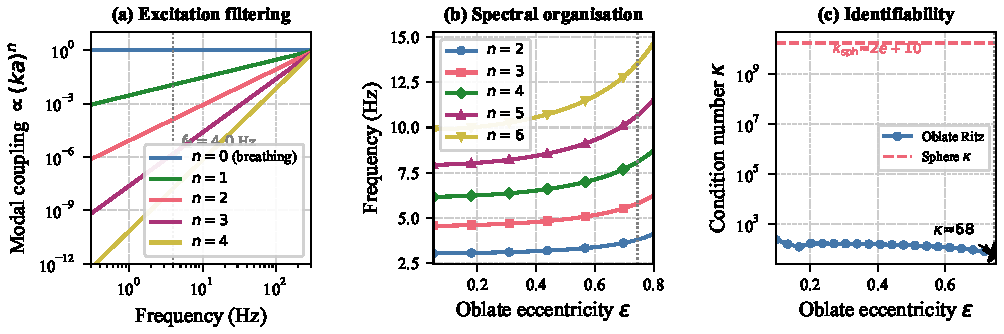
\includegraphics[width=\textwidth]{figures/fig_three_jobs.pdf}
  \caption{The three roles of geometry in fluid-filled shell mechanics:
    (a)~excitation filtering via $(ka)^n$ suppression,
    (b)~spectral organisation showing modal frequency dependence on eccentricity,
    (c)~identifiability improvement showing condition number reduction from
    sphere to oblate Ritz model.}
  \label{fig:three_jobs}
\end{figure}

The paper is organised as follows.  Section~\ref{sec:background} distils the
companion studies into the common geometric structure required for the present
argument.  Section~\ref{sec:theory} states and proves the formal results on
excitation filtering, rank collapse, asphericity-driven lifting, corrected
near-spherical asymptotics, and the forward--inverse adequacy gap.
Section~\ref{sec:results} assembles the principal numerical evidence across the
application classes.  Section~\ref{sec:discussion} interprets the results for
spectral inference on fluid-filled shells and emphasises the broader warning
against using forward success as a proxy for inverse reliability.
Section~\ref{sec:conclusion} closes with the central claim: in spectral inverse
problems on shells, geometry is not merely part of the model description; it is
the mechanism that decides what can be excited, what can be predicted, and what
can be inferred.
